\documentclass[a4paper,oneside,12pt]{book}
%% === nezbytné balíčky:
\usepackage[IL2]{fontenc}   % písmo pro UTF-8 || jiné: [T1] (funguje pro UTF-8?)
\usepackage[utf8]{inputenc} % vstupní znaková sada UTF-8 || [cp1250] -> Windows 1250 || [latin2] -> ISO Latin 2

\usepackage[czech]{babel} % česky psaná práce, typografická pravidla     

\usepackage{pdfpages} % pokud nemáte formulář "Zadání bak./dipl. práce" naskenovaný jako PDF, tak ZAKOMENTUJTE

%\usepackage{encxvlna} % postará se o spojky a předložky, které dle českých pravidel nesmí být na konci řádku. Dokumentace: http://texdoc.net/texmf-dist/doc/generic/encxvlna/encxvlna.pdf

\usepackage[a4paper, hmarginratio=1:1]{geometry} % využití celé A4 stránky a nastavení okrajů, pro OBOUSTRANNÝ TISK

%% === balíčky, které se mohou hodit:
\usepackage[hidelinks]{hyperref} % v PDF budou klikací odkazy ("hidelinks" je nebude rámovat)
\usepackage{graphicx} % balíček pro vkládání RASTROVÝCH grafických souborů (PNG apod.)
%\usepackage{epsfig} % balíčky pro vkládání VEKTOROVÝCH grafických souborů typu EPS

%\usepackage{float} % rozšířené možnosti umístění obrázků
%\usepackage{caption} % pro popisky obrázků, tabulek atd.

\usepackage{tabularx} % rozšířené možnosti tabulek
%\usepackage{tabu} % jiný balík pro rozšířené možnosti tabulek

\usepackage{listings}  % balíček vhodný pro ukázky kódu 
\usepackage{amsmath} % balíček pro pokročilou matematickou sazbu
%\usepackage{color} % pro možnost barevného textu
%\usepackage{fancybox} % umožňuje pokročilé rámečkování
%\usepackage{index} % nutno použít v případě tvorby rejstříku balíčkem makeindex
%\newindex{default}{idx}{ind}{Rejstřík} % zavádí rejstřík v případě použití balíku index


\topmargin=-15mm      % horní okraj trochu menší
\textwidth=150mm      % šířka textu na stránce
\textheight=240mm     % "výška" textu na stránce

\frenchspacing % za větou bude mezislovní mezera (v anglických textech je mezera za větou delší)
\widowpenalty=1000 % "síla" zákazu vdov (= jeden řádek odstavce na konci stránky)
\clubpenalty=1000 % "síla" zákazu sirotků (= jeden řádek/slovo odstavce samostatně na začátku stránky)
\brokenpenalty=1000 % "síla" zákazu zlomu stránky za řádkem, který má na konci rozdělené slovo

\pagenumbering{arabic} % číslování stránek arabskými číslicemi
\pagestyle{plain}      % stránky číslované dole uprostřed

\parindent=0pt % odsazení 1. řádku odstavce
\parskip=7pt   % mezera mezi odstavci

\newcommand{\ti}{\textit} % zkrácený příkaz pro kurzívu
\newcommand{\tb}{\textbf} % zkrácený příkaz pro tučné písmo


%% --- zde jsou makra, tj. "konstanty" - některé musíte změnit! --- %%
\newcommand{\cvut}{České vysoké učení technické v~Praze}
\newcommand{\fjfi}{Fakulta jaderná a fyzikálně inženýrská}
\newcommand{\katedra}{Katedra softwarového inženýrství}
\newcommand{\program}{Aplikace informatiky v~přírodních vědách} % změňte, pokud máte jiný stud. program
\newcommand{\spec}{--} % změňte, pokud studijní program má specializaci

\newcommand{\druh}{Diplomová práce} % nebo "Diplomová práce"
\newcommand{\woman}{} % pokud jste ŽENA, ZMĚŇTE na: ...{\woman}{a} (je to do Prohlášení)

\newcommand{\logoCVUT}{
\includegraphics{symbol_cvut_konturova_verze_cb.pdf}} % logo ČVUT -- podle grafického manuálu ČVUT platného od prosince 2016. Pokud nevyhovuje PDF-verze, tak použijte jinou variantu loga: https://www.cvut.cz/logo-a-graficky-manual -> "Symbol a logo ČVUT v Praze"). Pokud chcete logo úplně vynechat, zadejte místo "\includegraphics{...}" text "\vspace{35mm}"

% přesně podle formuláře "Zadání bak./dipl. práce" VYPLŇTE:
\newcommand{\nazevcz}{Český název práce}    % český název práce (přesně podle zadání!)
\newcommand{\nazeven}{Title}          % anglický název práce (přesně podle zadání!)
\newcommand{\autor}{Jméno Příjmení}   % vyplňte své jméno a příjmení (s akademickým titulem, máte-li jej)
\newcommand{\vedouci}{JménoV PříjmeníV} % vyplňte jméno a příjmení vedoucího práce, včetně titulů, např.: Doc. Ing. Ivo Malý, Ph.D.
\newcommand{\pracovisteVed}{\katedra, \fjfi, \cvut} % ZMĚŇTE, pokud vedoucí Vaší práce není z KSI
\newcommand{\konzultant}{--} % POKUD MÁTE určeného konzultanta, NAPIŠTE jeho jméno a příjmení + tituly
\newcommand{\pracovisteKonz}{--} % POKUD MÁTE konzultanta, NAPIŠTE jeho pracoviště

% podle skutečnosti VYPLŇTE:
\newcommand{\rok}{2023}  % rok odevzdání práce (jen rok odevzdání, nikoli celý akademický rok!)
\newcommand{\kde}{Praze} % studenti z Děčína ZMĚNÍ na: "Děčíně" (doplní se k "prohlášení")

\newcommand{\klicova}{Klíčová slova}   % zde NAPIŠTE česky cca 3-5 klíčových slov
\newcommand{\keyword}{Key words}       % zde NAPIŠTE anglicky cca 3-5 klíčových slov (přeložte z češtiny, ale odborně)
\newcommand{\abstrCZ}{Popis práce česky}    % zde NAPIŠTE abstrakt v češtině (alespoň 7 vět, min. 80 slov. Pokuste se, aby CZ i EN abstrakt nezpůsobily přetečení strany 6 na stranu 7, tj. aby se obojí i s klíčovými slovy vešlo na JEDNU stránku)
\newcommand{\abstrEN}{Popis práce anglicky} % zde NAPIŠTE abstrakt v angličtině

\newcommand{\prohlaseni}{Prohlašuji, že jsem svou bakalářskou práci vypracoval\woman{} samostatně a použil\woman{} jsem pouze podklady (literaturu, projekty, SW atd.) uvedené v přiloženém seznamu.} % text prohlášení můžete mírně upravit :-)

\newcommand{\podekovani}{Děkuji ... za ...} % NAPIŠTE poděkování, např. svému vedoucímu:
%"Děkuji Ing. Eleonoře Krtečkové, Ph.D. za vedení mé bakalářské práce a za podnětné návrhy, které ji obohatily."
% NEBO:
% Děkuji vedoucímu práce doc. Ing. Pafnutijovi Snědldítětikaši, Ph.D. za neocenitelné rady a pomoc při tvorbě bakalářské práce.


\begin{document}
%%%%%%%%%%%% TITULNÍ STRANA -- následujících cca 30 řádků se generuje AUTOMATICKY. Neměňte!!! Výjimka: práce psané v angličtině! %%%%%%%%%%%%
\thispagestyle{empty}

\begin{center}
    {\Large \textsc{\cvut}\\[4mm] \textsc{\fjfi}}\par
    \vspace{4mm}
	\tb{\katedra} \par\vspace{3mm}

    \begin{tabular}{l}
		\tb{Studijní program: \program}\\
		\tb{Specializace: \spec}\\
    \end{tabular}

   \vspace{10mm} \logoCVUT \vspace{15mm} 

   {\huge \tb{\nazevcz}\par}
   \vspace{5mm}   
   {\huge \tb{\nazeven}\par}
   
   \vspace{15mm}
   {\Large \MakeUppercase{\druh}}

   \vfill
   {\large
    \begin{tabular}{ll}
    Vypracoval: & \autor\\
    Vedoucí práce: & \vedouci\\
    Rok: & \rok
    \end{tabular}
   }
\end{center}

%%%%%%%%%%%% ZADÁNÍ PRÁCE %%%%%%%%%%%%
% Zadání (podepsané děkanem atd.) dostanou studenti KSI od sekretářky (nebo ji požádají, např. e-mailem).
\newpage  % SEM NESAHEJTE!
\thispagestyle{empty} % SEM NESAHEJTE!

%% naskenované ZADÁNÍ PRÁCE (nechte odkomentovanou jednu možnost!):
%% --- varianta A1: jednostránkové zadání v PDF:
%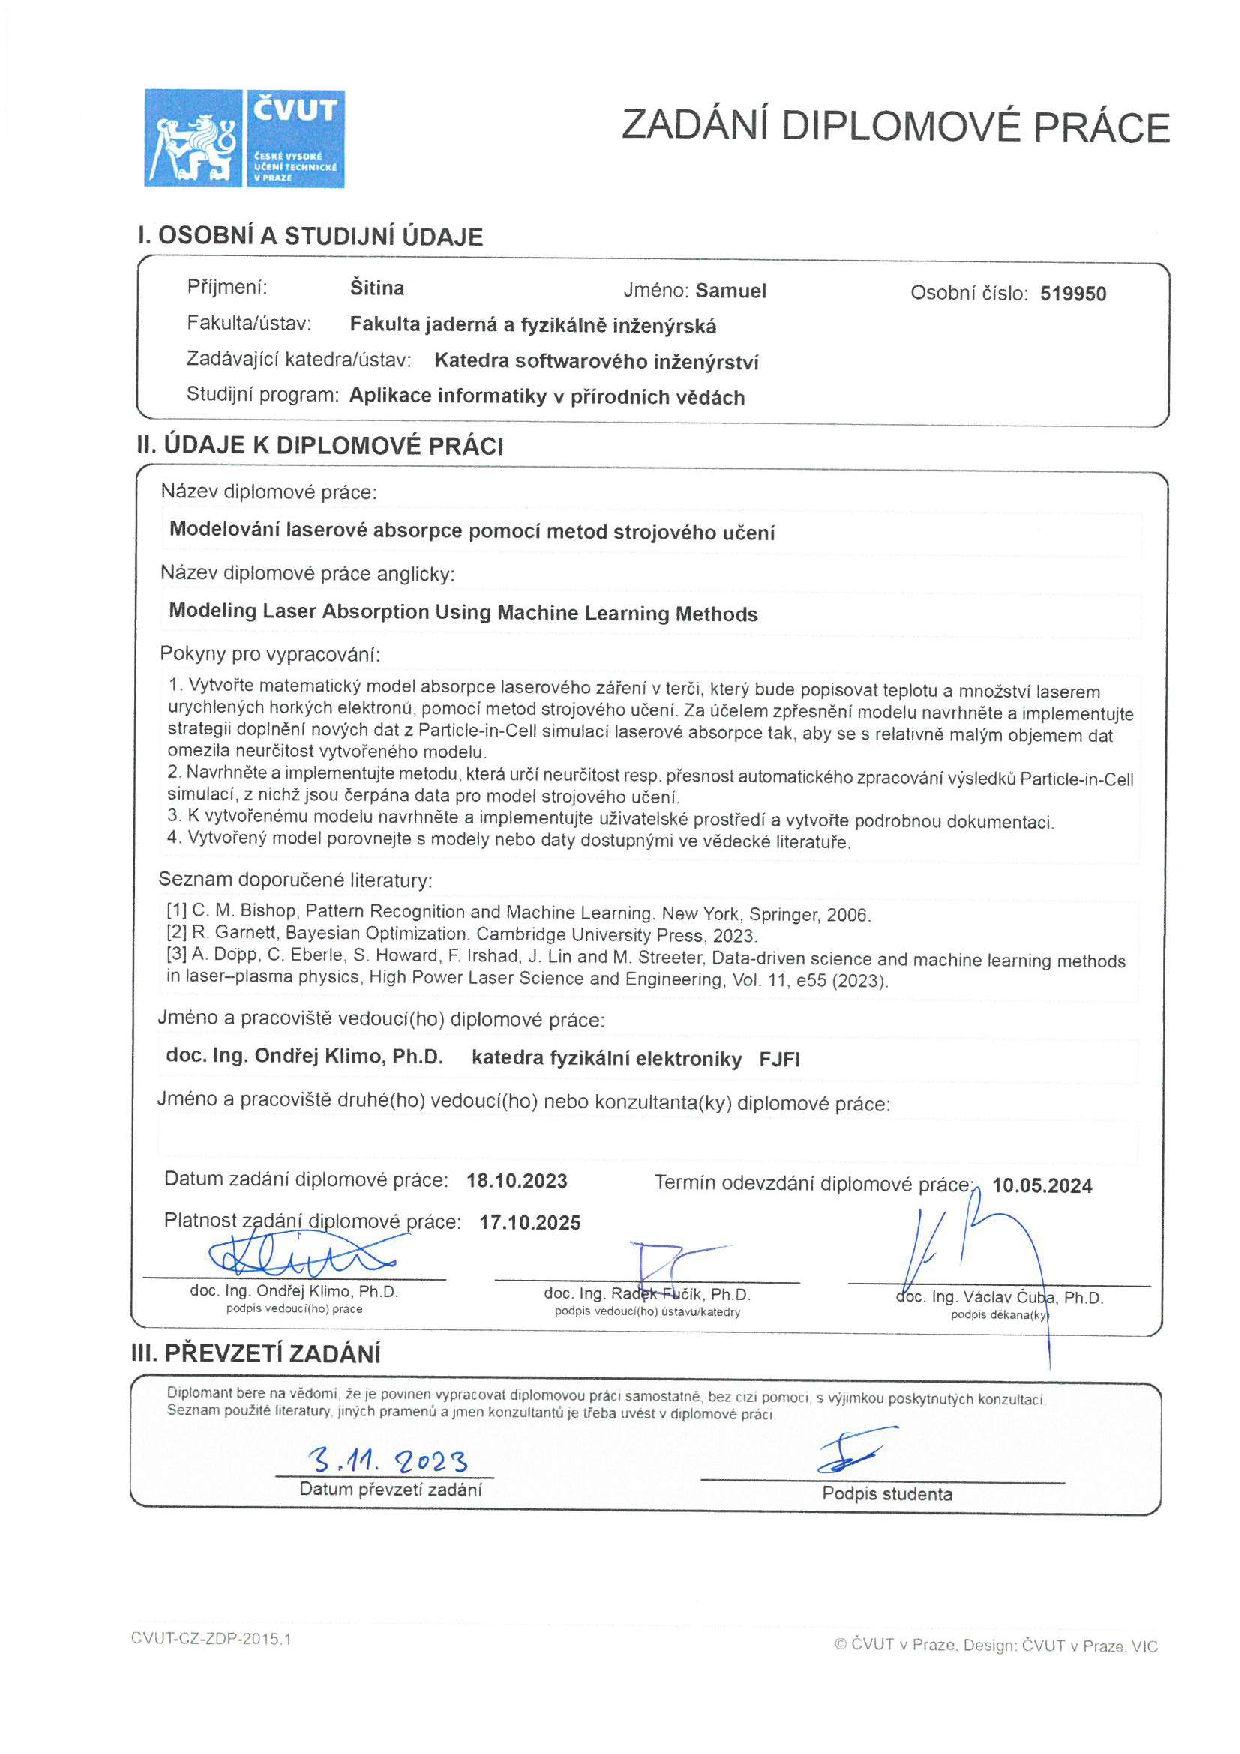
\includepdf[pages={1}]{zadani_cele.pdf} % A1) naskenováno do PDF
%% --- varianta A2: jednostránkové zadání v JPG:
%\begin{center}
%     \includegraphics[width=1\textwidth]{zadani1.jpg}
%\end{center}
%% --- varianta B1: dvoustránkové zadání v jediném PDF:
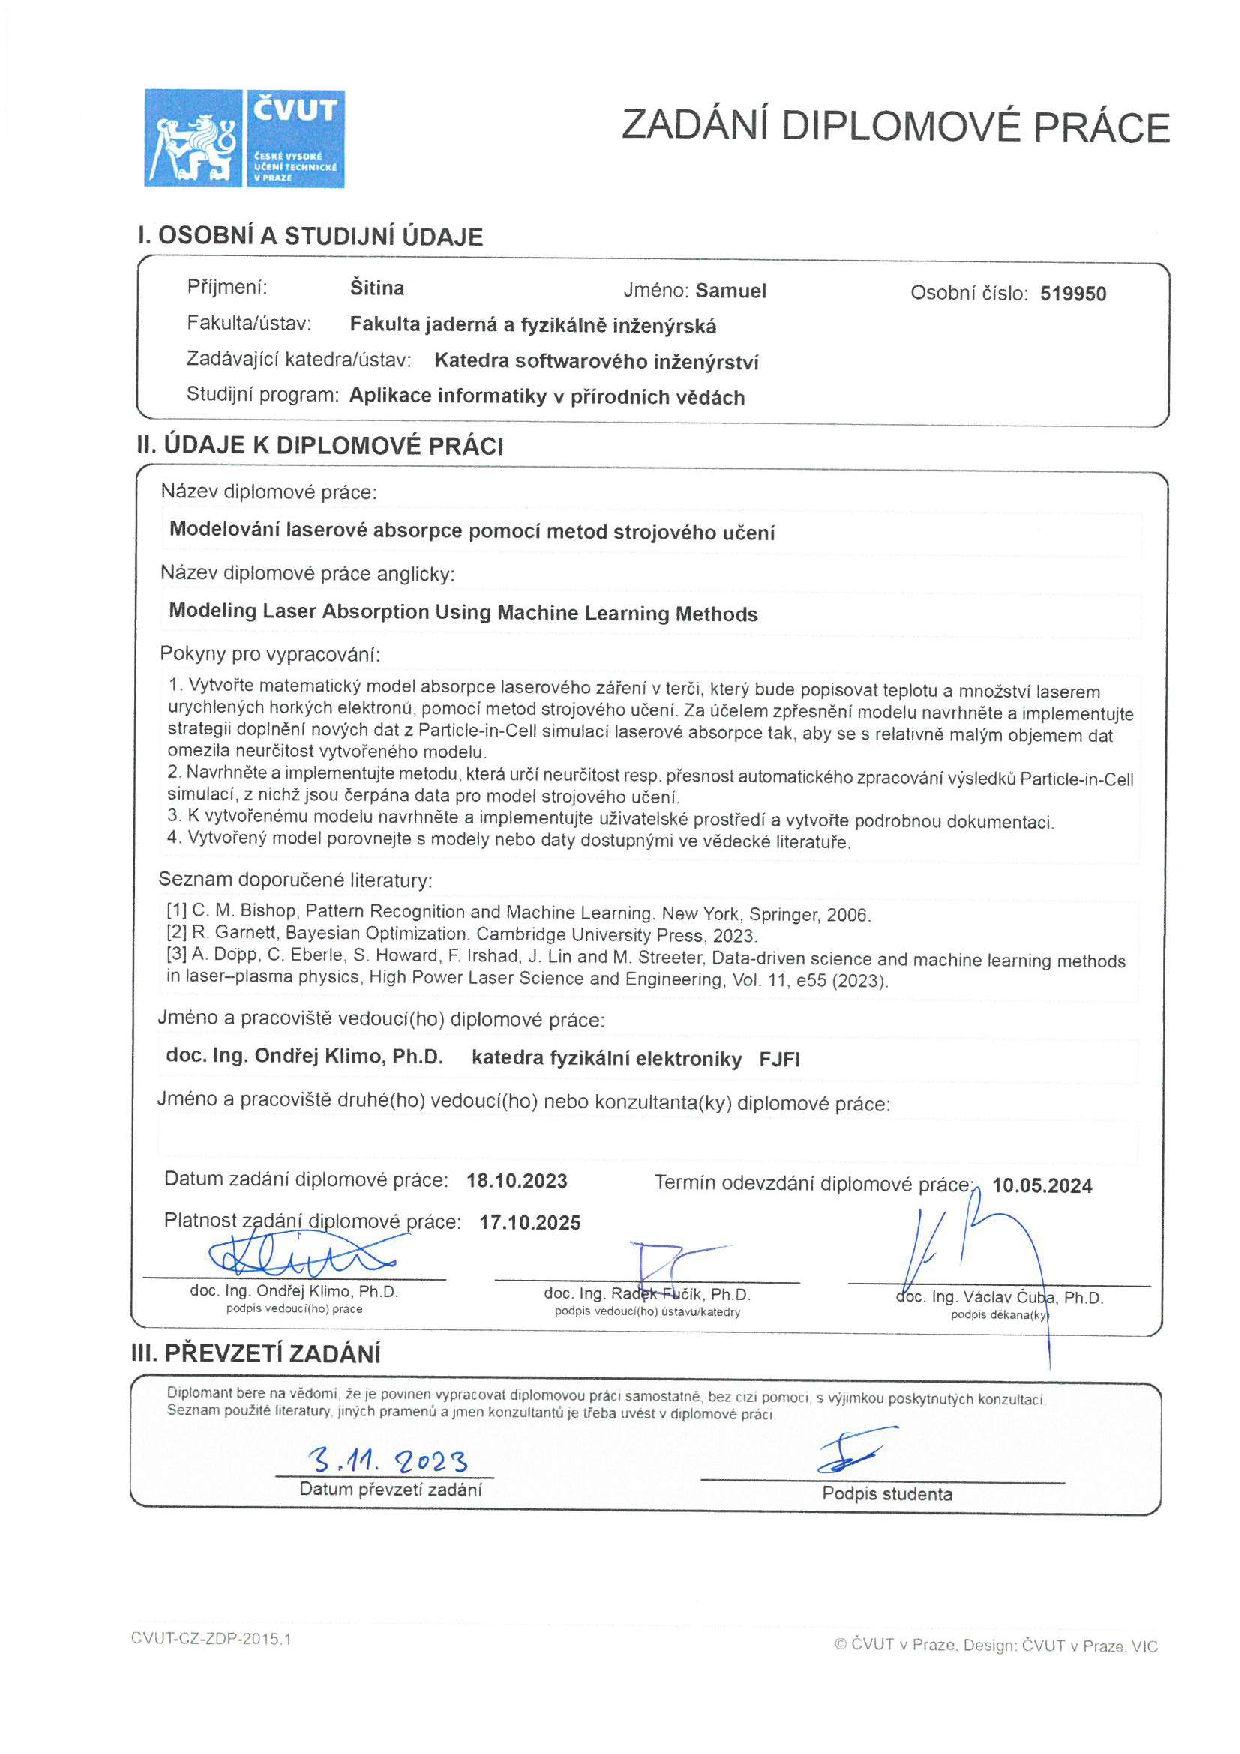
\includepdf[pages={1,2}]{zadani_cele.pdf} % PDF má 2 stránky
%% --- varianta B2: dvoustránkové zadání naskenované jako dvě samostatná jednostránková PDF:
%\includepdf[pages={1}]{zadani1.pdf} % 1. strana zadání v PDF
%\includepdf[pages={1}]{zadani2.pdf} % 2. strana zadání v PDF
%% --- varianta B3: dvoustránkové zadání naskenované jako dva samostatné JPG:
%\begin{center}
%     \includegraphics[width=1\textwidth]{zadani1.jpg} % 1. strana zadání
%\end{center}
%\newpage  
%\thispagestyle{empty}
%\begin{center}
%     \includegraphics[width=1\textwidth]{zadani2.jpg} % 2. strana zadání
%\end{center}
%% --- konec varianty B3


%%%%%%%%%%%% Prohlášení -- SEM NESAHEJTE! Generuje se automaticky z výše nastavených maker \kde{} a \prohlaseni{}. %%%%%%%%%%%%
\newpage % SEM NESAHEJTE!
\thispagestyle{empty}  % SEM NESAHEJTE!

~ % SEM NESAHEJTE!
\vfill % prázdné místo. SEM NESAHEJTE!

\tb{Prohlášení} % SEM NESAHEJTE!

\vspace{1em} % vertikální mezera. SEM NESAHEJTE!
\prohlaseni

\vspace{2em}  % SEM NESAHEJTE!
\hspace{-0.5em}\begin{tabularx}{\textwidth}{X c}  % SEM NESAHEJTE!
V \kde\ dne .................... &........................................ \\	% SEM NESAHEJTE!
	& \autor
\end{tabularx}	% SEM NESAHEJTE!


%%%%%%%%%%%% Poděkování -- tuto stránku můžete celou odstranit %%%%%%%%%%%%
\newpage
\thispagestyle{empty}

~
\vfill % prázdné místo

\tb{Poděkování}

\vspace{1em} % vertikální mezera
\podekovani
\begin{flushright}
\autor
\end{flushright}  % <------- tady končí stránka s poděkováním


%%%%%%%%%%%% ABSTRAKT atp. Je generován AUTOMATICKY podle maker nastavených na začátku souboru) %%%%%%%%%%%% 
\newpage   % SEM NESAHEJTE!
\thispagestyle{empty}   % SEM NESAHEJTE!

% příprava:    (na následujících 8 řádků NESAHEJTE!)
\newbox\odstavecbox
\newlength\vyskaodstavce
\newcommand\odstavec[2]{%
    \setbox\odstavecbox=\hbox{%
         \parbox[t]{#1}{#2\vrule width 0pt depth 4pt}}%
    \global\vyskaodstavce=\dp\odstavecbox
    \box\odstavecbox}
\newcommand{\delka}{120mm} % šířka textů ve 2. sloupci tabulky

% použití přípravy:    % dovnitř "tabular" vůbec NESAHEJTE!
\begin{tabular}{ll}
  {\em Název práce:} & ~ \\
  \multicolumn{2}{l}{\odstavec{\textwidth}{\bf \nazevcz}} \\[1em]
  {\em Autor:} & \autor \\[1em]
  {\em Studijní program:} & \program \\
  {\em Specializace:} & \spec \\
  {\em Druh práce:} & \druh \\[1em]
  {\em Vedoucí práce:} & \odstavec{\delka}{\vedouci\\ \pracovisteVed} \\
  {\em Konzultant:} & -- %\odstavec{\delka}{\konzultant \\ \pracovisteKonz}  % VYMAŽTE text "-- %" v případě, že jste neměli konzultanta
 \\[1em]  
  \multicolumn{2}{l}{\odstavec{\textwidth}{{\em Abstrakt:} ~ \abstrCZ  }} \\[1em]
  {\em Klíčová slova:} & \odstavec{\delka}{\klicova} \\[2em]

  {\em Title:} & ~\\
  \multicolumn{2}{l}{\odstavec{\textwidth}{\bf \nazeven}}\\[1em]
  {\em Author:} & \autor \\[1em]
  \multicolumn{2}{l}{\odstavec{\textwidth}{{\em Abstract:} ~ \abstrEN  }} \\[1em]
  {\em Key words:} & \odstavec{\delka}{\keyword}
\end{tabular}



%%%%%%%%%%%% Obsah práce ... je generován AUTOMATICKY %%%%%%%%%%%%
\newpage  % SEM NESAHEJTE!
\parskip=0pt
\tableofcontents % SEM NESAHEJTE!
\parskip=7pt
\newpage % SEM NESAHEJTE!


%--------------------------------------------------------
%|         Zde začíná SAMOTNÁ PRÁCE (text)              |
%--------------------------------------------------------

\chapter*{Úvod} % SEM NESAHEJTE!
\addcontentsline{toc}{chapter}{Úvod} % SEM NESAHEJTE!
%
Zde napište text úvodu (1-3 strany) nebo si text vložte ze samostatného souboru: např. příkazem \texttt{\textbackslash input\{vnitrek\_uvod.tex\}}.\par Text v~úvodu se nerozdělujte na podkapitoly, nýbrž na jednotlivé odstavce. Odstavce od sebe oddělíte prázdným řádkem nebo příkazem \texttt{\textbackslash par}. \par Úvod práce by měl obsahovat vymezení tématu práce (a~důvod výběru tématu), vymezení cíle/cílů práce, smysl cíle, způsob/metodu dosažení cíle (stručný nástin práce) a~předpoklady či omezení práce. Můžete čtenářům také nastínit strukturu práce (tj. co v~které kapitole najdou).
%
%\input{vnitrek_uvod.tex} % vložení souboru, který obsahuje text úvodu (bez nadpisu!)



\chapter{Jak psát závěrečnou práci} % změňte text kapitoly (pokud je \chapter součástí vkládaného souboru, tak tento řádek zakomentujte)
%
\small % zmenšení velikosti písma, aby pokyny byly kratší :-)
Tento text, vložený do \uv{šablony} příkazem \texttt{\textbackslash input\{vnitrek\_kapitola1.tex\}}, slouží jako stručné pokyny\footnote{Podrobnější informace o~psaní závěrečné práce získáte v~rámci předmětu \uv{Seminář k~bakalářské práci} (resp. \uv{Seminář k~diplomové práci}).} pro psaní závěrečné práce a~zároveň jej můžete využít jako ukázku práce v~\LaTeX{u}.
\par 
Ve skutečné závěrečné práci nahraďte soubor \texttt{vnitrek\_kapitola1.tex} za jiný (nebo kompletně přepište obsah souboru).

\newcommand{\prikaz}[1]{\texttt{\textbackslash #1\{\}}} % pomocné makro, definice by měla být spíše v preambuli, ale jelikož slouží pouze pro kapitolu~1 (a~ne pro všechny studenty), tak je umístěno zde

 
\section{Obsah textu}  
Obsah závěrečné práce musí zahrnovat všechny body z~osnovy (formulář \uv{Zadánín bak./dipl. práce}). Rozšíření zadání práce není zakázáno.
\par 
Textová část práce musí být {\em autorským dílem studenta} -- vyhýbejte se proto jakýmkoliv pokusům o~plagiátorství. Použité zdroje (knihy, webové stránky, software apod.) by měly být řádně citovány! Seznam použitých zdrojů se uvádí na konci práce, jednotlivé zdroje se citují příkazem \prikaz{cite}. Vyhněte se nejednoznačnostem a~nejasnostem v~textu.
\par
Teoretická část práce bývá v~rozsahu alespoň 10~stran. Z~textu musí být jasně patrné, co je převzato z~literatury a~co jsou původní myšlenky studenta. Teorie by měla souviset s~výsledkem závěrečné práce.
\par 
Praktická část práce by měla popsat/obsahovat dosažené výsledky (např. funkční program, číselný výsledek řešení, nové pravdivé řešení dokázané v~rámci teorie, objektivně zdůvodněné rozhodnutí). Konkrétní výsledek je zvýrazněn v~závěru práce a~bez teorie uvedené v~práci ho není možné dosáhnout. Výsledky práce by měly přinášet nějaké nové informace a~vlastní pohled studenta na zpracovávané téma.
\par
Samotná práce by měla být dobře strukturovaná a její jednotlivé části by na sebe měly {\em dobře logicky navazovat}. Důraz by měl být kladen na věcnost, odbornou úroveň, dobrou čtivost a~(je-li to možné) aktuálnost textu. Velmi důležitá je {\em faktická přesnost a~úplnost} (zejména při použití již neaktuálních zdrojů).
\par
{\bf Tip:} vyhněte se používání nevysvětlených zkratek. Nepoužívejte \uv{odbornou hantýrku}. Vyhněte se výrokům, které se dají různě interpretovat. Nepoužívejte příliš dlouhé věty. 



\section{Členění textu do kapitol a~sekcí}
Závěrečná práce obvykle obsahuje asi 5-6 kapitol (včetně úvodu a~závěru, tj. očíslované kapitoly jsou obvykle tři až čtyři). Kapitoly lze rozdělit na podkapitoly a~tyto dále na jednotlivé sekce:
\begin{itemize}
\item kapitola: {\texttt{\textbackslash chapter\{Název\}}},
\item podkapitola (v~kapitole): {\texttt{\textbackslash section\{Název\}}},
\item sekce (v~podkapitole):  {\texttt{\textbackslash subsection\{Název\}}}.
\end{itemize}
Dělení do nižších úrovní se nepoužívá (tak velký rozsah závěrečné práce nemají, aby byla potřeba další úroveň obsahu). 
\par
Názvy (pod)kapitol a~sekcí píšeme malými písmeny, kromě velkých začátečních písmen a~jmen (např. \uv{Trh v~České republice}). V~anglicky psané práci jsou pravidla jiná!
\par 
{\bf Tipy:} 
\begin{enumerate}
\item Je vhodné uložit si texty jednotlivých kapitol (nebo i~podkapitol) do samostatných souborů, neboť pak lépe/jednoduše přeskupíte vybrané části, když zjistíte, že původní obsah práce nebyl navržen vhodně. \par Typickým znakem nevhodně členěné práce jsou \uv{malé} (cca čtyřstránkové) kapitoly a~mezi nimi jedna \uv{velká} 20stránková kapitola.
\item Zdá se, že potřebujete čtvrtou úroveň členění? Zvažte, zda z~nějaké podkapitoly neudělat novou kapitolu závěrečné práce.
\item Pokud nevíte, jak vhodně rozčlenit svůj text, {\em požádejte o~radu vedoucího\/} své práce (při pravidelných konzultacích).
\end{enumerate}

\section{Obrázky a tabulky}\label{sekceObrTab}

Text závěrečné práce je vhodné doplnit tabulkami nebo obrázky (grafy, diagramy užití apod.), abyste lépe ilustrovali své myšlenky nebo dosažené výsledky. 
\par 
Obrázky a~tabulky se vkládají do plovoucího prostředí (\texttt{figure}, \texttt{table}). {\color{red} Plovoucí prostředí si LaTeX umístí sám} (na typograficky vhodné místo -- typicky nahoru či naopak dolů na stránku. Občas se obrázky dostanou až na konec kapitoly, ale nejedná se o~chybu).
\par 
Popis obrázku/tabulky se píše do příkazu \prikaz{caption} a~měl by být stručný a {\em výstižný}. Obrázky mají popis dole, kdežto tabulky mají popis nahoře. Pokud je obrázek (resp. tabulka) převzatý, nezapomeňte na konci popisku citovat zdroj!
\par 
Do textu vždy {\em napište důvod použití\/} obrázku/tabulky a~odkažte se na něj/ni:
\begin{itemize}
\item vytvoření odkazu: příkaz \prikaz{label} následovaný po příkazu \prikaz{caption},
\item sazba čísla odpovídajícího odkazu (tj. např. číslo obrázku): příkaz \prikaz{ref},
\item sazba čísla stránky, kde je odkaz: příkaz \prikaz{pageref}.
\end{itemize}   
Tabulky a~obrázky v~plovoucím prostředí používají své vlastní, {\em nezávislé číselné řady}. Z~toho vyplývá, že v~odkazech uvnitř textu musíme kromě čísla udat i~informaci o~tom, zda se jedná o~obrázek, anebo tabulku! Příklad: \texttt{vizte obrázek\textasciitilde\textbackslash ref\{odkazObrA\}}.
\par

\subsection{Obrázky}
Obrázky se vkládají do plovoucího prostředí \texttt{figure}. Nesnažte se přesvědčit \LaTeX, aby byl obrázek umístěný uprostřed stránky! Porušilo by to typografická pravidla sazby.\par 
Formát obrázku volte pokud možno vektorový (tj. EPS nebo PS), protože se dají zvětšovat i~zmenšovat bez újmy na čitelnosti. Pokud máte k~dispozici obrázek pouze v~rastrovém formátu (např. PNG nebo schéma v~JPG), nakreslete jej znovu v~některém vektorovém grafickém programu. Nemá smysl konvertovat bitmapové obrázky do formátu EPS.
\par 
{\bf Tip:} pomocí balíčku \href{https://texample.net/}{\underline{TikZ}} lze kreslit některé typy obrázků přímo v~textu práce. (Pro použití TikZ je potřeba přidat správný příkaz \prikaz{usepackage} v~preambuli \uv{šablony}.)

\subsubsection*{Ukázka -- kód pro vložení obrázku}
Příkazy pro vložení obrázku \texttt{graf.png}, na který se bude dát odkazovat pomocí \texttt{grafA}:
\begin{verbatim}
\begin{figure}
  \centering      % vycentrovat
  \includegraphics[scale=1]{graf.png} % soubor + měřítko (scale)
  \caption{Graf závislosti $y$ na $x$.} % popis obrázku
  \label{grafA} % definice odkazu na obrázek (pro \ref{})
\end{figure}
\end{verbatim}

\subsection{Tabulky} 
Tabulky se vkládají do plovoucího prostředí \texttt{table}. Součástí tohoto dokumentu je tabulka~\ref{tabMakra} (na straně~\pageref{tabMakra}), která obsahuje přehled maker ze \uv{šablony}.

\subsubsection*{Ukázka -- kód pro vložení tabulky}
Příkazy pro dvousloupcovou tabulku se záhlavím (tučně) a jedním řádkem, vše orámováno čarou (styl orámování tabulky si můžete zvolit, ale dodržujte stejný v~celé práci): 
\begin{verbatim}
\begin{table}
  \centering
  \caption{Popis tabulky.} 
  \label{odkazTabA} % odkaz na číslo tabulky, lze využít v \ref{odkaz}
  \begin{tabular}{|l|l|} % 2 sloupce, zarovnání obsahu doleva
    \hline \bfseries{název1} & \bfseries{název2}\\
    \hline data1 & data2 \\
    \hline % koncová čára
  \end{tabular}
\end{table}
\end{verbatim}


\section{Typografická pravidla}\label{podkapTypo}
Text práce musí vyhovovat typografickým pravidlům. Pokud netušíte, o~co jde, vyhledejte si např. heslo \uv{Základní pravidla hladké sazby}.
\par 
Především se zaměřte na:
\begin{itemize}\itemsep=2pt
\item {\bf členicí (interpunkční) znaménka} $\rightarrow$ podrobnosti pod heslem \uv{Pravopis -- interpunkce} na webu \url{https://prirucka.ujc.cas.cz/}.\par
Základní typografická pravidla pro znaménka:\\
Tečka, čárka, středník, dvojtečka, otazník a vykřičník se přimykají k~předcházejícímu slovu bez mezery (mezera se píše až za nimi). Výjimkou je desetinná čárka (v~anglicky psané práci desetinná tečka), okolo které se mezery nepíšou;
\item {\bf spojovník} (spojovací čárka) a~{\bf pomlčka}\footnote{Pomlčka v~anglicky psané práci se sází jako \texttt{-{}-{}-} a bez mezer okolo.} jsou různé znaky! Pro spojovací čárku píšeme znak \texttt{-}, kdežto pomlčku sázíme jako \texttt{-{}-}.\par 
Kdy (a~jak) se používá pomlčka: \url{https://prirucka.ujc.cas.cz/?id=165}.\par 
Kdy se používá spojovník: \url{https://prirucka.ujc.cas.cz/?id=164};
\item {\bf závorky} se přimykají k~vnitřnímu textu, tedy mezera se píše  před levou závorkou, a~pak za pravou závorkou;
\item \textbf{uvozovky} se přimykají k~vnitřnímu textu. V~česky psané práci můžete využít makro {\tt \textbackslash uv\{text\}}. 
\par
Pozor: pokud uvádíte ukázky zdrojového kódu programů, tak v~nich se používají uvozovky anglické (a také jiný typ písma).
\par Podrobnosti k~používání uvozovek: \url{https://prirucka.ujc.cas.cz/?id=162};
\item \textbf{apostrof} (odsuvník): \url{https://prirucka.ujc.cas.cz/?id=168};
\item \textbf{lomítko} jako oddělovač se píše bez mezer. Příklad: {\tt školní rok 2000/2001}; %
\item \textbf{procento} se sází se zpětným lomítkem. Pozor na rozdíl mezi 20\,\% (dvacet procent) a 20\% (dvacetiprocentní)! Podrobnosti: \url{https://prirucka.ujc.cas.cz/?id=790};
\item \textbf{pevná mezera} (znak {\tt \textasciitilde}) se píše mezi zkratkou jména a příjmením nebo mezi jednopísmennou předložkou/spojkou a~následujícím slovem. Mezi číslem a~jednotkou se píše {\bf úzká mezera}. Ukázka: {\tt 7.\textbackslash,11.\textbackslash,1811 se narodil K.\textasciitilde J.\textasciitilde Erben}.
\end{itemize}

\subsubsection*{Zvýrazňování textu}
Pro zvýraznění pojmů uvnitř textu se používá \textit{kurzíva} (příkaz \prikaz{textit} nebo lze využít makro \prikaz{ti} definované v~\uv{šabloně}).\par 
Silné zvýraznění (tj. tučné písmo) se v~závěrečných pracích uvnitř odstavců nepoužívá (nicméně existuje příkaz \prikaz{textbf} nebo makro \prikaz{tb} ze \uv{šablony}).


\subsubsection*{Psaní výčtů}
Pro psaní výčtů lze v~\LaTeX{u} využít prostředí {\tt enumerate} (číslovaný seznam) nebo {\tt itemize} (odrážky), položky píšeme do {\tt \textbackslash item}. Pravidla: \url{https://prirucka.ujc.cas.cz/?id=870}.


\subsubsection*{Psaní zkratek}
O~psaní zkratek pojednává heslo \uv{Zkratky, značky, čísla a~číslovky} na webovém rozcestníku \url{https://prirucka.ujc.cas.cz/}.

\subsubsection*{Složení čísel a slov}
Jak správně psát slova složená z~čísel a~slov? Vcelku podrobné vysvětlení naleznete na: \url{https://prirucka.ujc.cas.cz/?id=790}.\par 
Pozor na \textit{význam}: {\tt 5°} znamená pětistupňový, kdežto {\tt 5\,°} (s~úzkou mezerou) znamená pět stupňů.\par 
Ukázka správného zápisu (všimněte si: je to bez mezer a~bez spojovníku):\\
-- {\tt 20leté pozorování} nebo\\
-- {\tt dvacetileté pozorování} (jakékoli jiné tvary jsou chybné!).\par


\subsubsection*{Psaní značek}
Psaní značek, především matematických: \url{https://prirucka.ujc.cas.cz/?id=785}.


\section{Sazba matematického textu}

Mezi nejdůležitější typografické zásady psaní matematického textu patří:
\begin{itemize}\itemsep=2pt
\item známé konstanty a čísla určitá se píšou vzpřímeným řezem (např. $124$, $\mathrm e$, $\mathrm{\pi}$, $1-3\mathrm i$),
\item obecné konstanty a proměnné se píšou kurzívou (např. $a$, $x$, $x_1$),
\item identifikátory vektorů a matic se sázejí tučným řezem písma, např. $\mathbf{v}$, $\mathbf{M}$,
\item názvy funkcí (resp. známých polynomů) se píšou vzpřímeným řezem (např. $\sin(x)$, $\exp(y)$, $\mathrm{p}(x)$),
\item diferenciály se píšou vzpřímeným řezem, příslušná proměnná pak kurzívou: $\mathrm{d}x$.
\end{itemize}

Poznámka: příkazy pro matematickou sazbu jsou popsány též v~knize {\em \LaTeX pro začátečníky} od J.~Rybičky (ISBN 80-7302-049-1).


\subsection{Odkazy na rovnice nebo vztahy}
Rovnice, na které se budete v~textu odvolávat, opatřete pořadovými čísly při pravém okraji příslušného řádku (např. prostředí {\tt equation}). Příklad:
\begin{equation}\label{vzorec1}
p = \frac{1}{n}\cdot\sum_{i=1}^n c_i
\end{equation}

Číslování rovnic může být průběžné v~textu, nebo v~jednotlivých kapitolách, {\em odkaz na vzorec\/} vysází příkaz {\tt $\backslash$eqref\{odkaz\}} z~balíku {\tt amstex}, resp. napište: {\tt ($\backslash$ref\{odkaz\})}.
%Příklad: \hspace*{10mm} Průměrnou hodnotu z~čísel $c_1,c_2,\ldots,c_n$ vypočteme podle vztahu \eqref{vzorec1}.


\subsubsection{Desetinné číslo v~matematickém režimu} \label{des_cislo}
V českém textu používáme u~čísel desetinnou {\em čárku}, avšak čárka je v~mate\-ma\-tickém režimu
chápána jako oddělovač prvků seznamu ($\Rightarrow$ \LaTeX\ za ni automaticky přidává mezeru), proto je nutno desetinnou čárku uzavírat do složených závorek: {\tt \$a=21\{,\}7\$}.

\section{Ukázky zdrojových kódů}
Pokud chcete v~textu své práce upozornit na nějaký obzvláště zajímavý zdrojový kód\footnote{Veškeré zdrojové kódy svého programu odevzdáte jako samostatnou přílohu závěrečné práce v~systému KOS, typicky jako archiv (např. ZIP. Velikostní limit je asi 2~GB).}, můžete zařadit krátkou ukázku (obvyklejší však je, že ukázky zdrojového kódu uvedete až do textové přílohy práce s~patřičným komentářem. Nebo je neuvádíte do textu vůbec).

Prostředí pro zdrojové kódy: jednoduché {\tt verbatim} nebo pokročilejší {\tt lstlisting}, kde se zvýrazní syntaxe nastaveného programovacího jazyka (příkaz \prikaz{lstset}).


\section{Pravidla českého pravopisu}\label{sekcePravidla}
Text práce by se neměl prohřešit pravidlům českého pravopisu. Jako pomocník může posloužit např. \url{https://prirucka.ujc.cas.cz/}, kde nahoru napíšete slovo a necháte si jej vyhledat (zda vůbec takové slovo existuje a~jak se skloňuje/časuje, resp. jak se používá).
\par 
{\bf Tip:} nainstalujte si do editoru kontrolu {\em českého\/} pravopisu. Pokud si nejste čímkoli jisti, kupte/půjčte si aktuální \uv{Pravidla českého pravopisu} nebo požádejte o~kontrolu gramatických chyb osobu s~vytříbeným smyslem pro český jazyk (která se nebude zaměřovat na obsah práce, ale právě na stylistiku a pravopis).
\par
Pozor: není úkolem vedoucího práce, aby opravoval (a~četl) pravopisné chyby ve vašich \uv{betaverzích} textu! 


\section{Formátování seznamu použitých zdrojů}
% Stručně: https://prirucka.ujc.cas.cz/?id=883

Ve své závěrečné práci studenti pracují s~různými zdroji informací (ideálně s~knihami, nikoli nerecenzovanými weby). Text práce pak bude obsahovat údaje, které nejsou původní, a~proto je potřeba zdůraznit, co není studentův text:
\begin{itemize}
\item citují se použité {\em zdroje, které se týkají obsahu práce} (nikoli zdroje související s~úpravou/formou závěrečné práce, jako např. příručka k~\LaTeX u),
\item citován by měl být vždy {\em originální zdroj} (nikoli stránka z~Wikpedie). Pokud se jedná o~nějaký všeobecně známý fakt, normu, resp. standard de facto či de iure, tak není potřeba hledat zdroj;
\item seznam použitých zdrojů je umístěn za závěrem práce a~{\color{red} řadí se abecedně podle příjmení autorů} (pokud autor chybí, tak podle prvního slova).
\end{itemize}

Pravidla pro práci s~bibliografickými citacemi jsou definována českými technickými normami ČSN~ISO~690 a~690-2.
\par {\bf Tip:} použijte \url{https://www.citacepro.com/} a vyexportujte si uložené zdroje do TeXu (před exportem abecedně seřaďte dle příjmení autorů!)
\par 
Dbejte na {\em úplnost} použitých zdrojů $\Rightarrow$ uvádějte co nejvíce informací o~citovaném zdroji (např. název sborníku, číslo stránky ve sborníku, platný odkaz na článek). \par
Pozor: web CitacePro nemusí obsahovat relevantní informace o~použitém zdroji $\Rightarrow$ vždy si citaci zkontrolujte podle originální knihy!

%\cite{iso690,iso690-2}, z~nichž vycházejí také srozumitelnější formou psané dokumenty \cite{kra05,bold1,bold2,vym01}. 





\section{Křížové odkazy} \label{kap-odkazy}
Pro odkazy na stránky, na čísla kapitol a podkapitol, na čísla obrázků a tabulek atd. využíváme
speciálních prostředků DTP programu, které zajistí vygenerování správného čísla i~v případě, že se
text posune díky změnám samotného textu nebo díky úpravě parametrů sazby. V~systému \LaTeX\ jde o~odkaz na číslo, které odpovídá umístění značky v~textu (tzv. navěští).

\subsubsection{Definice návěští}

Návěští se definuje pomocí {\tt \textbackslash label\{navesti\}}\footnote{V seznamu použitých zdrojů se návěští definuje jinak: {\tt $\backslash$bibitem\{id\}}.\label{poznBibitem}}, uvedeného \underline{za} příkazem pro vytvoření objektu (např. u~obrázku za příkazem \prikaz{caption}, u~podkapitoly za příkazem \prikaz{section}).\par 
{\color{red} Návěští musí být v~rámci celého dokumentu {\em jedinečné}} -- na nejednoznačnosti upozorní {\LaTeX} při překladu dokumentu (+ zprávy se ukládají do LOG-souboru)!
\par 
Každé návěští se vztahuje k~nějakému čítači (coun\-ter), např. k~číslu kapitoly, podkapitoly, obrázku či tabulky. Můžete si také definovat vlastní prostředí
s~čítačem (příkaz \prikaz{newcounter}).

\subsubsection{Odkaz na návěští}
Použití odkazu závisí na tom, co potřebujete:
\begin{enumerate}
\item {\tt $\backslash$ref\{navesti\}} ... vysází odkaz na návěští, tj. vytiskne hodnotu příslušného čítače v~daném místě (např. {\em číslo} kapitoly nebo {\em číslo} obrázku).\par 
Pozor: příkaz netiskne název objektu(!) $\Rightarrow$ musíte napsat, od čeho je to číslo, např.: {\tt na {\color{red}obrázku}\textasciitilde \textbackslash ref\{obrXY\} je znázorněn průběh teplot};
%
\item {\tt$\backslash$pageref\{navesti\}} ... vysází \textit{číslo stránky}, kde se nachází odkazovaná položka;
\end{enumerate}
Speciality:
\begin{itemize}
\item {\tt $\backslash$eqref\{navesti\}} ... odkaz na číslo rovnice/vzorce (nutný balíček {\tt amsmath}); %
\item {\tt $\backslash$cite\{id\}} ... odkaz na položku ze seznamu použitých zdrojů$^{\ref{poznBibitem}}$.
\end{itemize}


\section{Finální úpravy před odevzdáním práce}

Závěrečná práce se odevzdává elektronicky v~systému KOS (termíny odevzdání jsou určeny harmonogramem akademického roku na FJFI).
\par
Před odevzdáním výsledného PDF si zkontrolujte (resp. nechte si od někoho zkontrolovat):
\begin{itemize}
\item zda je vloženo správné (podepsané) oficiální zadání práce + první strany práce mu odpovídají  ($\Rightarrow$ máte správně vyplněná makra z~tabulky~\ref{tabMakra});
\item jestli text práce neobsahuje gramatické (podkapitola~\ref{sekcePravidla}) nebo stylistické chyby,
\item zda v~práci nejsou typografické chyby (podkapitola~\ref{podkapTypo}). Pozor: často zůstávají na konci řádků jednopísmenné předložky/spojky,
\item jestli práce neobsahuje formální či věcné chyby (takovéto problémy pomůže odhalit vedoucí práce, kterému {\color{red} dostatečně včas\/} před termínem odevzdání práce {\color{red} několikrát} ukážete svůj text).
\end{itemize}




\begin{table}[h]
\centering
{\footnotesize
\caption{Makra definovaná v~\uv{šabloně} (v~abecedním pořadí).}\label{tabMakra}
\begin{tabular}{|l|l|l|}
\hline {\bfseries makro} & {\bfseries význam} & {\bfseries jak vyplnit} \\ 
\hline
\hline \prikaz{abstrCZ} & český popis práce (abstrakt) & vlastní text\\
\hline \prikaz{abstrEN} & anglický popis práce (abstract) & vlastní text\\ 
\hline \prikaz{autor} & \parbox{80mm}{\vspace{2px}\par jméno a příjmení autora závěrečné práce, včetně dosavadních titulů\par\vspace{3px}} & dle zadání! \\
\hline \prikaz{cvut} & oficiální název vysoké školy & dle zadání! \\
\hline \prikaz{druh} & typ závěrečné práce & dle zadání!\\
%\verb{\druh{Diplomová práce}} \\
\hline \prikaz{fjfi} & oficiální název fakulty & dle zadání!\\
\hline \prikaz{kde} & místo odevzdání (6. pád $\Rightarrow$ \uv{Praze} nebo \uv{Děčíně}) & místo studia\\
\hline \prikaz{keyword} & klíčová slova (anglicky) oddělená čárkou & vlastní text\\ 
\hline \prikaz{klicova} & klíčová slova (česky) oddělená čárkou & vlastní text\\
\hline \prikaz{konzultant} & jméno a příjmení konzultanta & dle zadání \\ % \footnotemark[\ref{pozn}]
\hline \prikaz{katedra} & oficiální název katedry & dle zadání!\\
\hline \prikaz{logoCVUT} & logo ČVUT (lev s~kružítkem) & neměnit!\\
\hline \prikaz{nazevcz} & český název práce & dle zadání!\\
\hline \prikaz{nazeven} & anglický název práce & dle zadání! \\
\hline \prikaz{podekovani} & text poděkování & vlastní text\\
\hline \prikaz{pracovisteKonz} & pracoviště konzultanta & dle zadání! \\
\hline \prikaz{pracovisteVed} & pracoviště vedoucího práce & dle zadání! \\
\hline \prikaz{program} & název studijního programu & dle zadání!\\
\hline \prikaz{prohlaseni} & text prohlášení & vlastní text\\
\hline \prikaz{rok} & konkrétní rok odevzdání práce (nikoli celý akad. rok) & dle skutečnosti\\
\hline \prikaz{spec} & název specializace (pokud ji váš studijní program má) & dle zadání! \\
\hline \prikaz{tb} & zvýraznění tučným písmem (zkratka příkazu \prikaz{textbf}) & neměnit\\
\hline \prikaz{ti} & zvýraznění kurzívou (zkratka příkazu \prikaz{textit}) & neměnit\\
\hline \prikaz{vedouci} & jméno a příjmení vedoucího práce, včetně titulů & dle zadání! \\
\hline \prikaz{woman} & koncovka minulého času u~sloves & \uv{a} pro ženy\\
%muž: \verb{\woman{}}, žena: \verb{\woman{a}} \\
\hline 
\end{tabular}
}
\end{table}

{\color{blue}Poznámka: případné chyby v~tomto textu pište na e-mail  {\tt dana.majerova(at)fjfi.cvut.cz}.} % text vkládán ze souboru. Pokud je v souboru uveden i příkaz \chapter{...}, tak ho o 2 řádky výše vymažte!


\chapter*{Závěr}
\addcontentsline{toc}{chapter}{Závěr} % SEM NESAHEJTE!
%
Zde napište text závěru své práce (1-3 strany, nerozdělujte na podkapitoly) nebo jej vložte ze samostatného souboru: např. příkazem \texttt{\textbackslash input\{vnitrek\_zaver.tex\}}. \par Závěr by měl obsahovat shrnutí práce a~zopakovat/zdůraznit, jaké jsou výsledky. Může obsahovat i~náměty na budoucí rozšířené práce. \par V~závěru práce byste neměli hodnotit svou práci -- to udělají členové komise při státní závěrečné zkoušce.
%
%\input{vnitrek_zaver.tex}


%%%%%%%%%%%% SEZNAM POUŽITÝCH ZDROJŮ (LITERATURA) %%%%%%%%%%%%
\clearpage
\addcontentsline{toc}{chapter}{Seznam použitých zdrojů} % SEM NESAHEJTE!
\begin{thebibliography}{99}   
% následující text (2 řádky) zaměňte citacemi svých zdrojů
	\bibitem{odkaz} Autor. \ti{Název knihy}. Město. Nakladatelství. Rok. 
\end{thebibliography}
% formát: ČSN ISO 690. Můžete si to vygenerovat na http://www.citacepro.com (přihlaste se přes odkaz "ČVUT"), umí to vygenerovat TeX
% řazení: abecedně podle autora (resp. provního slova, není-li znám autor)


%%%%%%%%%%%% PŘÍLOHY PRÁCE %%%%%%%%%%%%
\newpage % SEM NESAHEJTE!
\addcontentsline{toc}{chapter}{Přílohy} % SEM NESAHEJTE!
\appendix % SEM NESAHEJTE!


%%%%%%%%%%%% Příloha A (tj. 1. kapitola v rámci příloh) %%%%%%%%%%%%
\chapter{Název přílohy} % zde změňte název přílohy, příp. zakomentujte a vložte soubor, kde je název přílohy + její text (odmažte/zakomentujte text níže + odkomentujte \input{}):
Zde napište text první přílohy nebo jej vložte, např.: \texttt{\textbackslash input\{priloha\_A.tex\}}.
%
%\input{priloha_A.tex} % text vkládán ze souboru, kde je i příkaz \chapter{...}


\end{document} % SEM NESAHEJTE! Konec.
